\documentclass[11p]{article}
% Packages
\usepackage{amsmath}
\usepackage{graphicx}
\usepackage[swedish]{babel}
\usepackage[
    backend=biber,
    style=authoryear-ibid,
    sorting=ynt
]{biblatex}
\usepackage[utf8]{inputenc}
\usepackage[T1]{fontenc}
%Källor
\addbibresource{mall.bib}
\graphicspath{ {./images/} }

\title{PMmall \\ \small Fysik 1}
\author{Magnus Silverdal }
\date{\today}

\begin{document}

    \begin{titlepage}
        \begin{center}
            \vspace*{1cm}

            \Huge
            \textbf{Title}

            \vspace{0.5cm}
            \LARGE
            Subtitle

            \vspace{1.5cm}

            \textbf{Milton Långström}

            \vfill

            Ett PM om energiförsörjning \\
            Fysik 1

            \vspace{0.8cm}

            
\includegraphics[width=0.4\textwidth]{NTI Gymnasiet_Symbol_print_svart}

            \Large
            Teknikprogrammet\\
            NTI Gymnasiet\\
            Umeå\\
            \today

        \end{center}
    \end{titlepage}
% Om arbetet är långt har det en innehållsförteckning, annars kan den utelämnas
    \tableofcontents
    \newpage

    \section{Inledning}
    Att diskutera kärnkraft är viktigt eftersom det är en kontroversiell energikälla som påverkar många olika aspekter av vårt samhälle.

    Kärnkraft kan generera stora mängder el utan att släppa ut stora mängder växthusgaser, vilket kan hjälpa till att minska vår koldioxidavtryck.

    Samtidigt finns det också potentiella risker med kärnkraft, såsom olyckor och avfallshantering.


    \subsection{frågeställningar}
    \begin{enumerate}
        \item Hur fungerar ett kärnkraftverk?
        \item Vilka miljöpåverkan har ett kärnkraftverk lokalt och globalt?
        \item Hur påverkar kärnkraft samhället (Ekonomi/politik/konflikter/m.m.) lokalt och globalt?
    \end{enumerate}

    \section{Resultat}

    \subsection{Så fungerar kärnkraftverk}
    Ett kärnkraftverk skapar elektricitet genom att man kokar massiva mängder vatten vilket i sin tur gör så att en turbin som är kopplad till en generator roterar.
    Vattnet inuti reaktorn kokas genom att man klyver atomer vilket sätter igång en kedjereaktion som värmer vattnet, denna kedjereaktion kallas för en fissionkedja.
    De atomer som klyvs i kärnkraftverk är oftast uran-235 eftersom att det är det grundämne som lättast att klyva, uran-235 är även ett väldigt radioaktivt ämne.
    \parencite{Vattenfall}
    \begin{figure}[!h]
        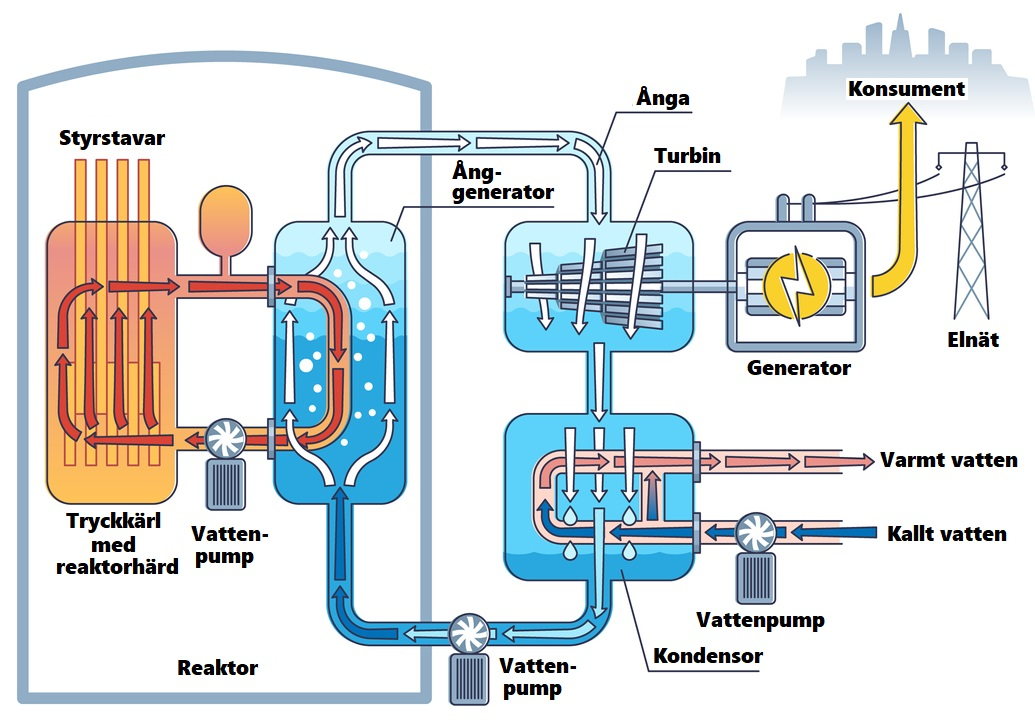
\includegraphics[width=0.8\textwidth]{karnkraftverk-2}
        \caption{Förenklad bild utav hur ett kärnkraftverk fungerar Källa : Ugglans fysik}
        \label{bild}
    \end{figure}
    \printbibliography

    \subsection{Globala miljökonsekvenser av kärnkraft}
    Kärnkraftverk höjer även vatten temperaturen eftersom att kylvattnet som används i anläggningarna oftast kommer ifrån sjöar eller hav, då detta vatten släpps ut igen så har temperaturen på vattnet ökat med 10 celsius.
    \parencite{Naturvårdsverket}

    Denna höjning på 10 celcius kan innebära stora skador på de marina ekosystem som är i det uppvärmda vattnet  \textcite{Energiforsk}


    Vid en härddsmälta så kan flera städer bli obeboliga i flera miljoner år pågrundutav att uran-235 har en halveringstid på 710 miljoner år. \textcite{Strålsäkerhetsmyndigheten2}


    \subsection{Lokal miljöpåverkan av ett kärnkraftverk}
    Finns inte så jätte många lokala nackdelar till kärnkraft förutom de minimala mängder radioaktiva material som släpps ut från kraftverken. Kärnkraftverk tar även upp stora områden utav land.
    \subsection{Såhär påverkar ett kärnkraftverk naturen}
    Kärnkraft anses vara en av de renaste energikällorna eftersom den har mycket lägre koldioxidutsläpp jämfört med kraftverk som drivs av olja, kol eller gas.


    De utsläpp som dock kommer ifrån kärnkraftverk är små mängder utav radioaktiva ämnen, dessa ämnen består utav kortlivade radioaktiva ämnen vilket leder till att radioaktiviteten minskar relativt snabbt. \parencite{Naturvårdsverket}

    \subsection{Hur påverkar kärnkraften samhället?}
    Kärnkraft är en energikälla som påverkar samhället på många olika sätt, både positivt och negativt. Kärnkraften bidra till att minska koldioxidutsläppen och därför hjälpa till att minska de massiva koldioxid utsläpp som vi har inom dagens samhälle.

    Kärnkraften kan också ge ekonomiska fördelar genom att skapa arbetstillfällen och öka energiförsörjningen.

    Å andra sidan finns det risker med kärnkraft som kan påverka samhället negativt. Kärnkraftsolyckor kan orsaka skada på miljön och hälsan, påverka turism, jordbruk och fiske.

    Kärnkraft kan också vara en politiskt fråga som kan skapa konflikter mellan länder, särskilt när det gäller kärnvapen. Därför är det viktigt att noga överväga kärnkraftens potentiella risker.
\parencite{Nationalgeographic}

    \section{Slutsatser}
    De slutsatser jag själv kommit fram till i detta pm är att kärnkraft är en väldigt effektiv och ren energikälla.


    Dock så finns det stora risker som kommer med att använda kärnkraft, där dem flesta utav dem innebär massförstörelse där chernobyl är ett bra exempel.


% Mer saker som du kan ha nytta av.





\end{document}
